\documentclass[11pt, a4paper,oneside,chapterprefix=false]{scrbook}

\usepackage{a4wide}
\usepackage{times}
\usepackage{helvet}   % sets sans serif font

\usepackage{amsmath,amssymb,amsthm}

\usepackage{graphicx}
\usepackage{subfigure}  
\usepackage{fancybox} % for shadowed or double bordered boxes
\usepackage{fancyhdr}
\usepackage{mdframed}

\DeclareGraphicsExtensions{.pdf, .jpg}

%% macros
 \def\mathbi#1{\textbf{\em #1}}
 
% commands
\newcommand{\Adjoint}{\mbox{\rm Adj}}
\newcommand{\Area}{\mbox{\rm Area}}
\newcommand{\ACos}{{\mbox{\rm Cos}^{-1}}}
\newcommand{\ASin}{{\mbox{\rm Sin}^{-1}}}
\newcommand{\ATan}{{\mbox{\rm atan2}}}
\newcommand{\Code}[1]{{\tt #1}}
\newcommand{\Complex}{\mbox{\bf C}}
\newcommand{\Cross}{{\mbox{\rm Cross}}}
\newcommand{\Mydddot}[1]{\mbox{\shortstack{$.$\hspace*{-1pt}$.$\hspace*{-1pt}$.$\\$#1$}}}
\newcommand{\Degree}{\mbox{\rm degree}}
\newcommand{\Diag}{\mbox{\rm Diag}}
\newcommand{\Dim}{\mbox{\rm dim}}
\newcommand{\Dist}{\mbox{\rm Distance}}
\newcommand{\IntTwo}{\int\!\!\int}
\newcommand{\IntThree}{\int\!\!\int\! \!\int}
\newcommand{\Kernel}{\mbox{\rm kernel}}
\newcommand{\Kross}{\mbox{\rm Kross}}
\newcommand{\Grad}{\nabla}
\newcommand{\Perp}{\mbox{\rm Perp}}
\newcommand{\Point}[1]{{\cal #1}}
\newcommand{\Rank}{\mbox{\rm rank}}
\newcommand{\Range}{\mbox{\rm range}}
\newcommand{\Real}{{\mbox{\rm I}\hspace*{-2pt}\mbox{\rm R}}}
\newcommand{\RealSbt}{{\mbox{\rm\scriptsize I}\hspace*{-2pt}\mbox{\rm\scriptsize R}}}
\newcommand{\Res}{\mbox{\rm resultant}}
\newcommand{\Sbt}[1]{{\mbox{\rm\scriptsize #1}}}
\newcommand{\MySign}{\mbox{\rm Sign}}
\newcommand{\SignSBT}{\mbox{\rm\scriptsize Sign}}
\newcommand{\Skew}{\mbox{\rm Skew}}
\newcommand{\Span}{\mbox{\rm Span}}
\newcommand{\SqrDist}{\mbox{\rm Distance$^2$}}
\newcommand{\Trace}{\mbox{\rm Trace}}
\newcommand{\TRN}{{\mbox{\rm\scriptsize T}}}
\newcommand{\Vector}[1]{\mbox{\bf #1}}
\newcommand{\VectorM}[1]{\mbox{\boldmath $#1$}}
\newcommand{\Volume}{\mbox{\rm Volume}}

\newcommand{\IVec}{\mbox{\boldmath $\imath$}}
\newcommand{\JVec}{\mbox{\boldmath $\jmath$}}
\newcommand{\KVec}{\mbox{\boldmath $k$}}
\newcommand{\LVec}{\mbox{\boldmath $\ell$}}
\newcommand{\RMat}{{\cal R}}
\newcommand{\QMat}{{\cal Q}}
\newcommand{\QCMat}{\overline{\cal Q}}

\newcommand{\Lerp}{\mbox{\rm lerp}}
\newcommand{\Slerp}{\mbox{\rm slerp}}
\newcommand{\Quad}{\mbox{\rm quad}}
\newcommand{\Squad}{\mbox{\rm squad}}

\newcommand{\ODer}[2]{\frac{d #1}{d #2}}
\newcommand{\ODerT}[2]{\frac{d^2 #1}{d {#2}^2}}
\newcommand{\ODerM}[3]{\frac{d #1}{d #2 \, d #3}}
\newcommand{\PDer}[2]{\frac{\partial #1}{\partial #2}}
\newcommand{\PDerT}[2]{\frac{\partial^2 #1}{\partial {#2}^2}}
\newcommand{\PDerM}[3]{\frac{\partial^2 #1}{\partial #2 \, \partial #3}}

% mass density symbol
\newcommand{\Den}{\delta}

% environments
\newenvironment{BArray}[1]{\left\{ \begin{array}{#1}}{\end{array} \right\}}
\newenvironment{Combin}{\left( \begin{array}{c}}{\end{array} \right)}
\newenvironment{Matrix}[1]{\left[ \begin{array}{#1}}{\end{array} \right]}


\let\mbf=\mathbf
\let\mvec=\mathbf
\let\mcal=\mathcal
\let\mfunc=\mathrm

%\def\R{\mbox{\ensuremath{\mathrm{I\!R}}}}
\newcommand{\R}{\ensuremath{\mathbb{R}}}
\newcommand{\N}{\ensuremath{\mathbb{N}}}
\newcommand{\Z}{\ensuremath{\mathbb{Z}}}
\newcommand{\C}{\ensuremath{\mathbb{C}}}

\newcommand{\of}[1]{\left( #1 \right)}
\newcommand{\abs}[1]{\left| #1 \right|}
\newcommand{\norm}[1]{\left\Vert {#1} \right\Vert}
\newcommand{\gradient}[1]{\nabla{\!}_{#1}{\,}}
\newcommand{\twovec}[2]{\left( #1 \atop #2 \right)}
\newcommand{\threevec}[3]{\left(\begin{array}{c}#1\\#2\\#3\end{array}\right)}
\newcommand{\fourvec}[4]{\left(\begin{array}{c}#1\\#2\\#3\\#4\end{array}\right)}

\newcommand{\refsec}[1]{Section~\ref{sec:#1}}
\newcommand{\reffig}[1]{Fig.~\ref{fig:#1}}
\newcommand{\reftab}[1]{Tab.~\ref{tab:#1}}
\newcommand{\refeq}[1]{Eq.~(\ref{eq:#1})}

%\newcommand{\R}{\hspace*{0.1ex}{\sf I} \hspace{-0.3ex}{\sf R}}

%6.5
\newcommand{\eps}{\mbox{$\epsilon$}}
\newcommand{\dmin}{\mbox{$d_{\min}$}}
\newcommand{\dmax}{\mbox{$d_{\max}$}}
\newcommand{\dminmax}{\mbox{$[\dmin,\dmax]$}}

%4.2:
\def\M{\mathcal{M}}
\def\n{\mathbi{n}}
\def\p{\mathbi{p}}
\def\q{\mathbi{q}}
\def\x{\mathbi{x}}
\def\tp{^{\mathsf{T}}}

\let\vec=\mathbi%
\let\mat=\mathbf%
\let\set= \mathcal%

% Taken from (and slightly modified): http://stackoverflow.com/questions/741985/latex-source-code-listing-like-in-professional-books

\usepackage{listings}
\usepackage{courier}
\usepackage{color}
\definecolor{lightgray}{gray}{0.9}
\definecolor{commentgreen}{rgb}{0.2,0.56,0.2}
 \lstset{
         basicstyle=\footnotesize\ttfamily, % Standardschrift
         numbers=left,               % Ort der Zeilennummern
         numberstyle=\tiny,          % Stil der Zeilennummern
         %stepnumber=2,               % Abstand zwischen den Zeilennummern
         numbersep=5pt,              % Abstand der Nummern zum Text
         tabsize=2,                  % Groesse von Tabs
         extendedchars=true,         %
         breaklines=true,            % Zeilen werden Umgebrochen
         keywordstyle=\color{red},
                frame=b,         
          keywordstyle=[1]\textbf,    % Stil der Keywords
         keywordstyle=[2]\textbf,    %
         keywordstyle=[3]\textbf,    %
         keywordstyle=[4]\textbf,   %\sqrt{\sqrt{}} %
         stringstyle=\color{blue}\ttfamily, % Farbe der String
         showspaces=false,           % Leerzeichen anzeigen ?
         showtabs=false,             % Tabs anzeigen ?
         xleftmargin=17pt,
         framexleftmargin=17pt,
         framexrightmargin=5pt,
         framexbottommargin=4pt,
         backgroundcolor=\color{lightgray},
         showstringspaces=false,      % Leerzeichen in Strings anzeigen ?
         commentstyle=\color{commentgreen}
 }
 \lstloadlanguages{% Check Dokumentation for further languages ...
         %[Visual]Basic
         %Pascal
         %C
		PHP, 
         C++
         %XML
         %HTML
         %Java
 }
    %\DeclareCaptionFont{blue}{\color{blue}} 

  %\captionsetup[lstlisting]{singlelinecheck=false, labelfont={blue}, textfont={blue}}
  \usepackage{caption}
\DeclareCaptionFont{white}{\color{white}}
\DeclareCaptionFormat{listing}{\colorbox[cmyk]{0.43, 0.35, 0.35,0.01}{\parbox{\textwidth}{\hspace{15pt}#1#2#3}}}
\captionsetup[lstlisting]{format=listing,labelfont=white,textfont=white, singlelinecheck=false, margin=0pt, font={bf,footnotesize}}

\usepackage{color}
\usepackage{hyperref}
\definecolor{RED}{rgb}{1,0,0}
\definecolor{GREEN}{rgb}{0,0.7,0}
\definecolor{BLUE}{rgb}{0,0,1}
\definecolor{Orange}{rgb}{0.7,0.7,0.7}
\newcommand{\FIXME}[1]{{\color{RED}{\textbf{FIX}: #1}}}

\addtolength{\textheight}{2.0cm}
\addtolength{\voffset}{-1cm}
\addtolength{\textwidth}{1.8cm}
\addtolength{\hoffset}{-.9cm}

\widowpenalty=10000
\clubpenalty=10000

%\author{Hans Muster}
%\title{Blockwise Hierarchical Data Decompositions}
%\date{Fall Semester 2011}

\begin{document}

\frontmatter
%\maketitle %automatic version
% --- selfmade version ----
\begin{titlepage}
	\setlength{\parindent}{0cm}
	\addtolength{\textheight}{1.0cm}

	\vspace{0.5cm}
	\Huge
	{\textbf \textsf{VIAN\\ \huge Visual Film Annotation and Analysis}}

	\vfill\vfill\vfill
	\vfill
	\includegraphics*[width=1.0\textwidth]{figures/vian_02.png}
	\vfill \vfill \vfill
	\large
	Author:\\
	Gaudenz Halter\\
	
	
	
	


	\begin{minipage}[b]{0.5\textwidth}
	ERC Advanced Grant FilmColors\\
	Department of Film Studies \\
	University of Z{\"u}rich
	\end{minipage}
	%
	\begin{minipage}[b]{0.5\textwidth} \raggedleft
	Visualization and MultiMedia Lab \\
	Department of Informatics \\
	University of Z{\"u}rich
	\end{minipage}

	\vfill
	\hrule
	\vspace{0.5cm}
	\includegraphics*[width=0.3\textwidth]{figures/uzh_logo} \hfill
	\includegraphics*[width=0.3\textwidth]{figures/vmml_logo}

\end{titlepage}
%%


%=====================================================================
\section{FilmColors Project} \label{chp:introduction}
%=====================================================================
VIAN is developed a part of the ERC FilmColors project, which aims to systematically investigate the relationships between technological processes and the aesthetics of film colors through a new interdisciplinary approach of film and computer science. The project will develop new software to analyze a large number of color films from each decade since the invention of film. Aesthetic analyses in film history will be supplemented with measurement methods from the natural sciences to investigate the chemical and physical characteristics of film colors.  \\
Part of the project is the segmentation and classification of a corpus of approximately 450 films. The process for each movie is the following: 

\begin{itemize}
	\item Segment a Film into coherent segments (ELAN)
	\item Taking a set of representing stills for each segment (ELAN)
	\item Classifying the Segments based on a large set of Vocabularies (FileMaker) (approx. 1000 words)
	\item Using (semi-)automatic tools to extract color-features (VIAN)
\end{itemize}

Most of these tasks have been done using ELAN for the segmentation and still-taking of the films. Since the number of stills per full-length movie lies roughly between 500 and 1000, storing each still separately and naming it correctly, can become a time-consuming process and involves a high error rate in the naming convention. As such, VIAN has initially been developed as an application that could be remotely controlled by ELAN and allowed to automatically generate stills, name them according to our convention, store them consistently and to be able to draw basic shapes onto a frame. 
Over the last year, the list of requirements for VIAN has grown, including: 

\begin{itemize}
	\item Providing an Interface for automatic analyses
	\item Per Frame Update when scrubbing though a movie
	\item Generating film visualizations
\end{itemize}

VIAN tries to simplify this process by combining all features needed in the described workflow. This is especially important for the FilmColors project, because one final product of the project should be a WebApp that allows visualization of the Corpus as well as a crowd-sourcing toolset that is able to commit new project to the Corpus. This toolset is VIAN. 


 
\newpage
%=====================================================================
\section{Entities} \label{chp:features}
%=====================================================================

The basic concept is, that there are entities that are collected by the user. (Segments, Visual Annotations and Screenshots), these can later be classified using a set of vocabularies. \\
To give an impression on how VIAN works and looks, some of the features are subsequently described. 

\subsection{Segmentation}
VIAN uses two types of Tier based annotations, Segmentations and Visual Annotations. Segments refer to annotations that don’t have a visual representation on the films frame, thus these are equivalent to the annotations of ELAN. 

\subsection{Visual Annotations}
Contrary, visual annotations have an additional representation on the screen, i.e. Text, Image, basic geometric shapes or freehand drawing. Their position and size may vary over time (\textit{keyable}). 

\begin{figure}[htp]
	\centering
	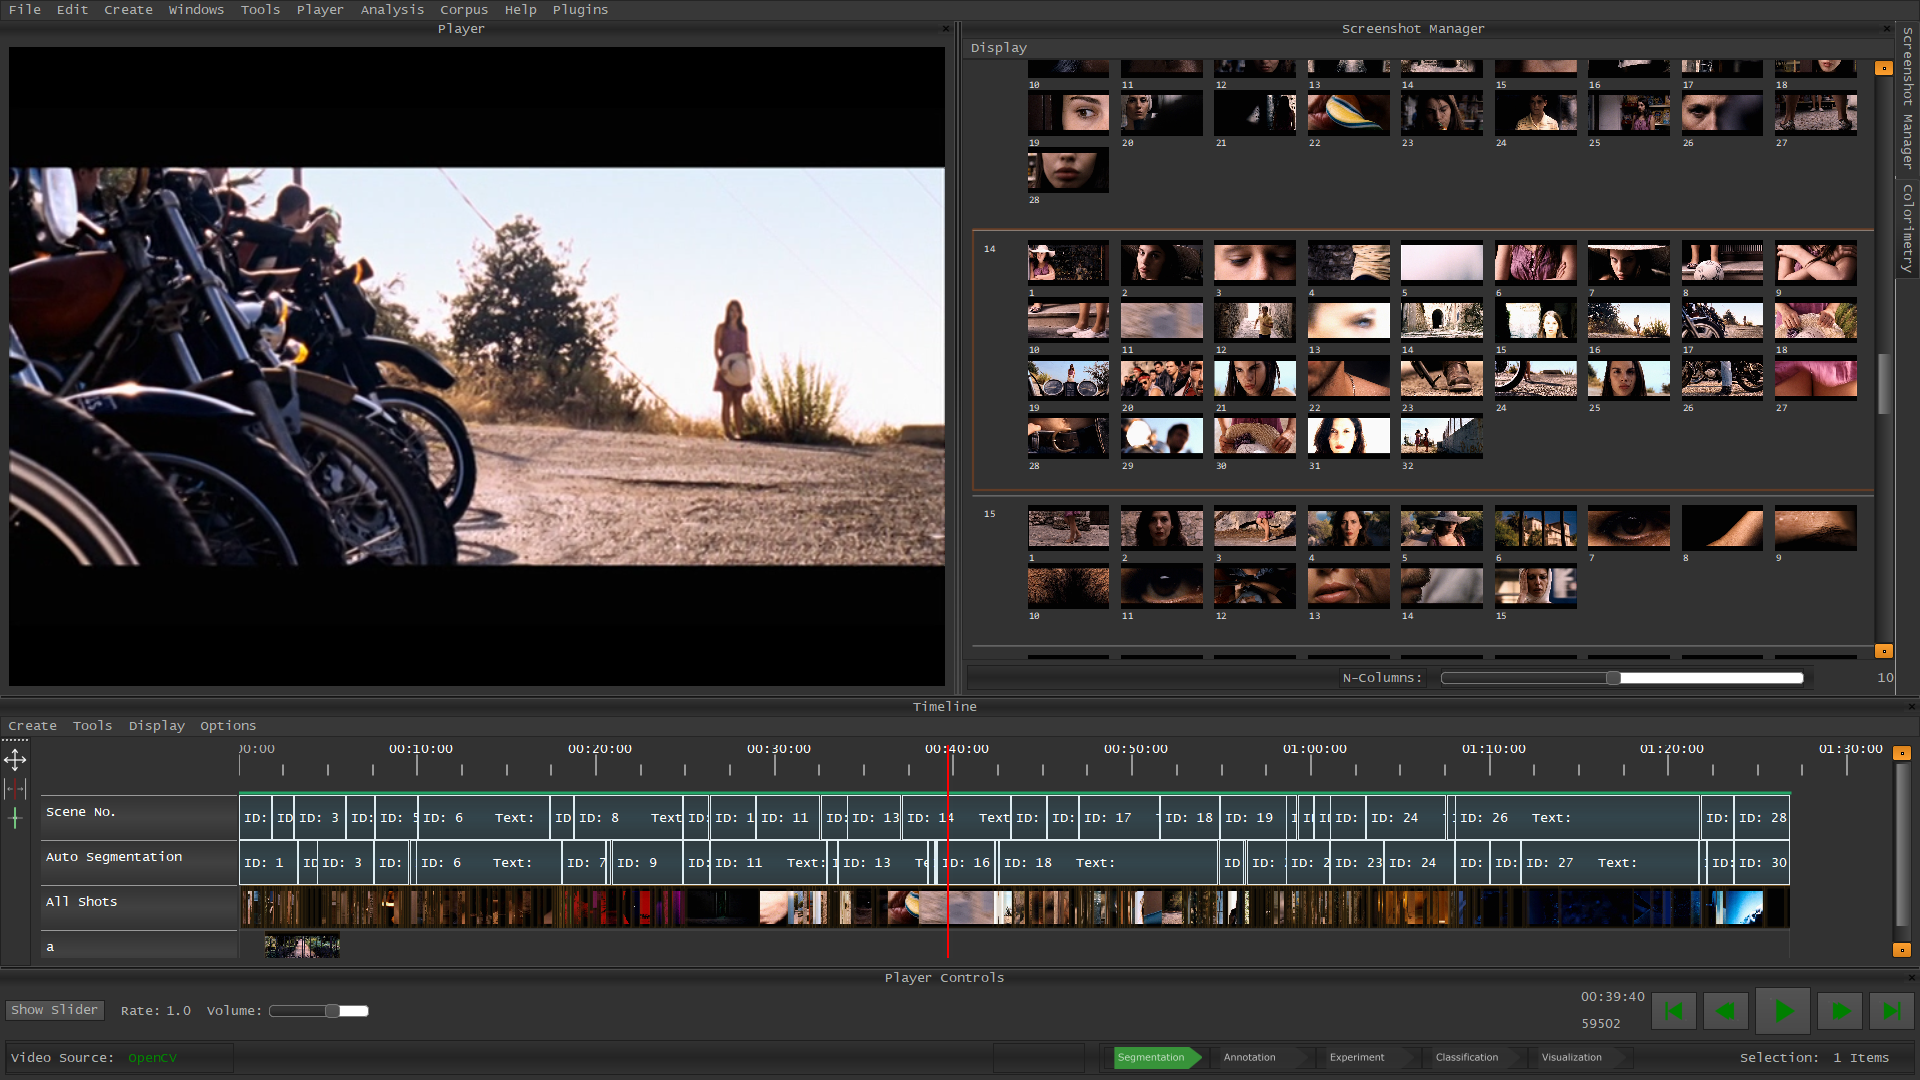
\includegraphics[width=1.0\textwidth]{figures/vian_segmentation.PNG}
	\caption{The default view of VIAN. The Screenshot Manager on the right. Stills are sorted by the segmentation and indexed within the segment. Additionally they are shown in the timeline. }
	\label{fig:vian_segmentation}
\end{figure}

\subsection{Screenshots}
VIAN treats stills as important objects, makes it easy to create, export and manage them. Typically, the stills represent a specific feature of a segment that the annotating person has observed. VIAN sorts them according to the segment they are in. Stills are only stored only by time, thus must  be exported to be accessible without VIAN. 

\subsection{External Media-Objects}
For both, annotations and segments, external media can be attached by simply drag and drop the file on the target in the timeline. VIAN will then copy the file to the project directory and link the media file to the entity it has been dropped. Once the user wants to open the file, VIAN tries to use the default application of the OS to open the file. 


\subsection{Experiments}

Once the Entities are collected, classification can set place. This is done using VIAN’s Experiment entity, which defines a set of rules that the annotator must conform. 

\begin{itemize}
	\item Automatic analyses that have to be performed (and their parameters)
	\item A list of Classification Objects and their associated Vocabularies
	\item Which entities should be classified
	\item The final classification results. (A list of keyword and entities)
\end{itemize}

Example: \\
In the FilmColors project, there is a specific distinction between \textit{foreground} (the character-space) and the background (the object-space and void). One vocabulary called “Hues” was used to classify the most dominant colors of both the foreground and background. Thus the Classification Objects are \textit{foreground} and \textit{background}, both have to be classified by the vocabulary “\textit{Hue}”.\\
A second vocabulary “\textit{Materials Character}” was used, to give information about what materials were used for clothing and jewelry of the characters. Since this vocabulary should only be applied to the characters, only the Classification Object “\textit{foreground}” should be classified by it.  In the VIAN Experiment editor this would look the following:

\begin{figure}[htp]
	\centering
	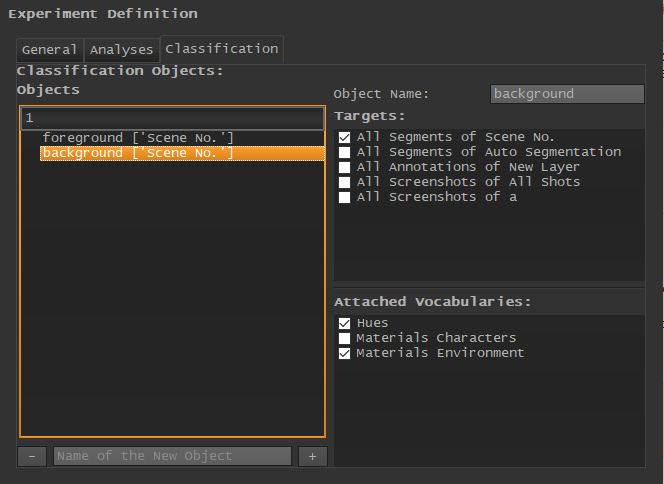
\includegraphics[width=0.48\textwidth]{figures/vian_exp_bg.png}
	\hfill
	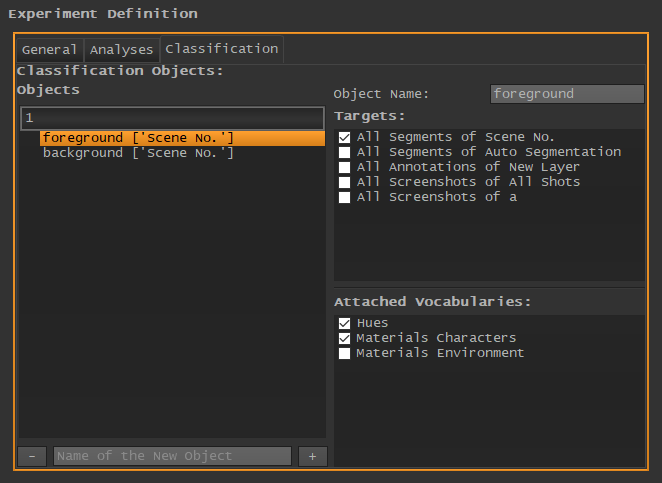
\includegraphics[width=0.48\textwidth]{figures/vian_exp_fg.png}
	\caption{The default view of VIAN. The Screenshot Manager on the right. Stills are sorted by the segmentation and indexed within the segment. Additionally they are shown in the timeline. }
	\label{fig:vian_classobj}
\end{figure}

\newpage
Once the experiment is setup, VIAN will loop through all entities that should be classified and show the user the corresponding vocabularies. 

\begin{figure}[htp]
	\centering
	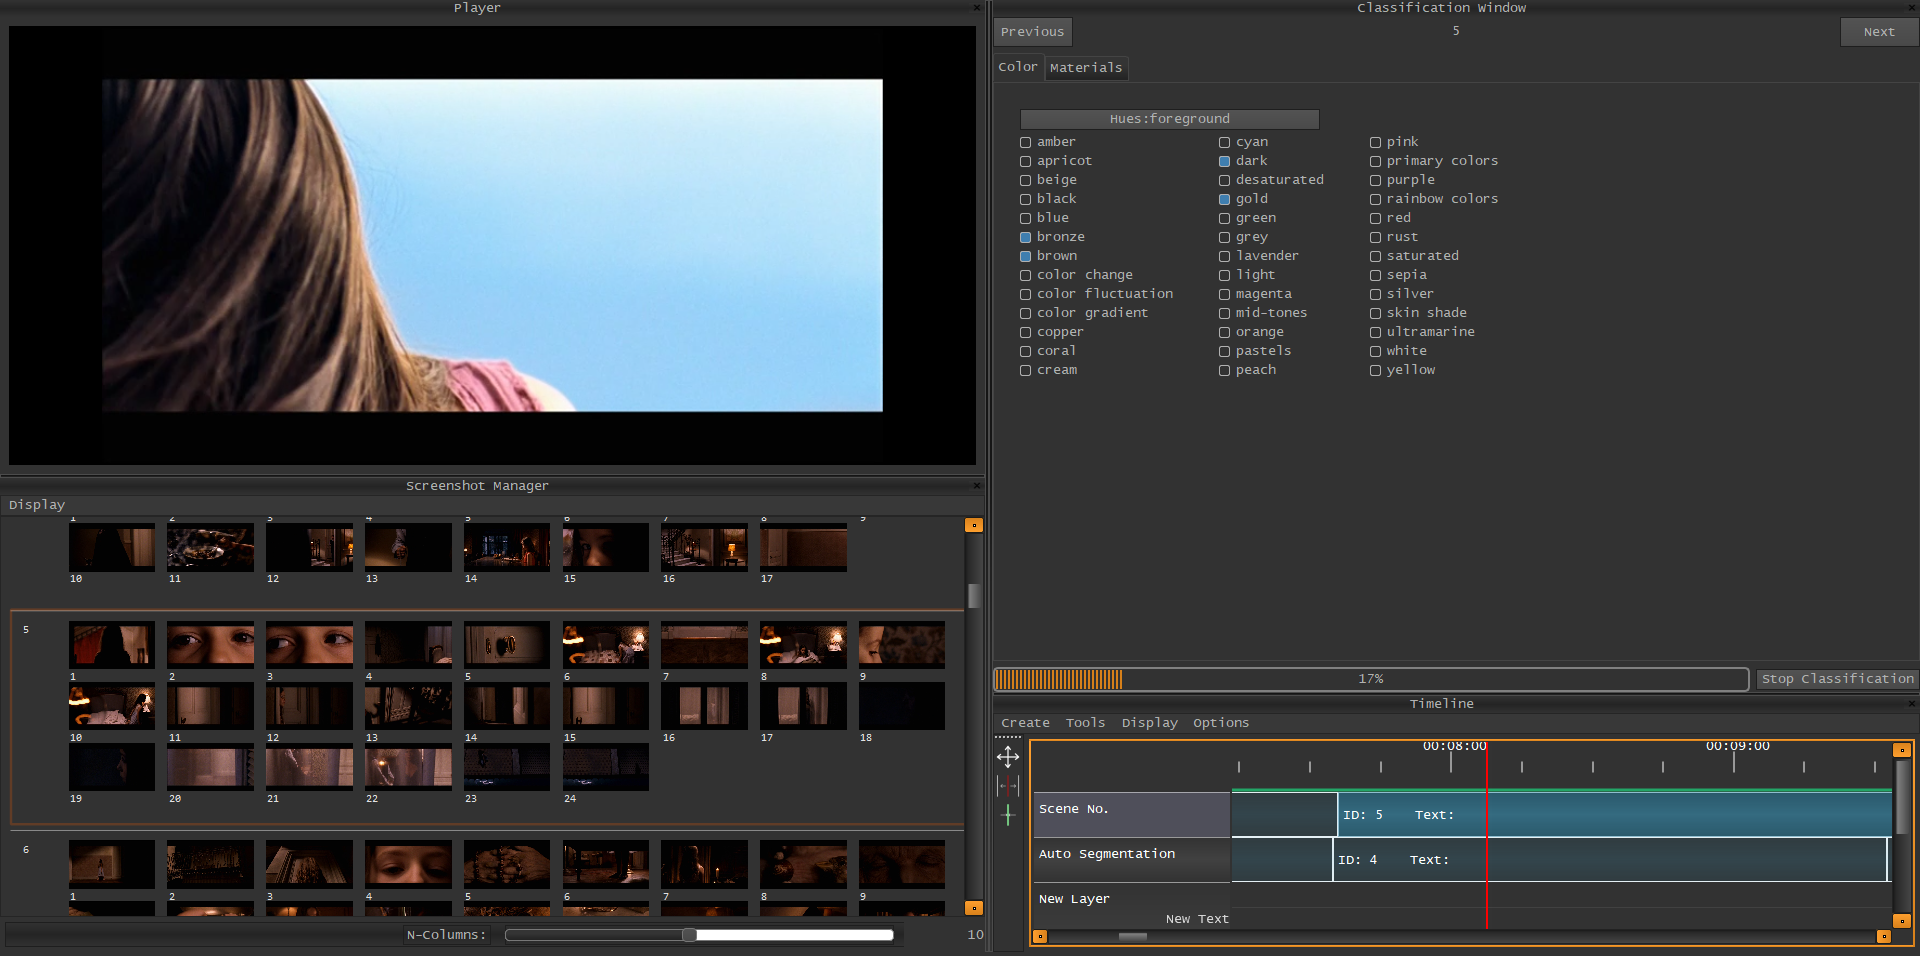
\includegraphics[width=1.0\textwidth]{figures/classification.PNG}
	\caption{The default view of VIAN. The Screenshot Manager on the right. Stills are sorted by the segmentation and indexed within the segment. Additionally they are shown in the timeline. }
	\label{fig:vian_classobj}
\end{figure}


\end{document}
